% !TEX root=/home/tavant/these/manuscript/src/manuscript.tex

\section{PIC simulation results: Coche model}

Now, the results from Coche' model

\subsection{Coche model: Temporal evolution} \label{subsec-temp_coche}

\begin{figure}[hbtp]
  \centering
  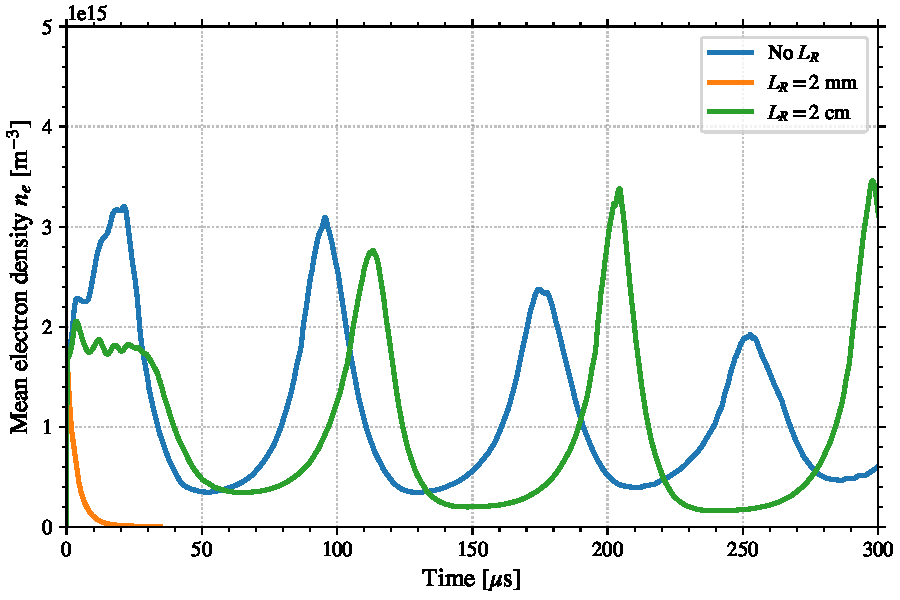
\includegraphics[width=\defaultwidth]{Coches_mean_ne}
  \caption{Temporal evolution of the average plasma density}
  \label{fig-coche_mean_ne}
\end{figure}

We can see in \Cref{fig-coche_mean_ne} the temporal evolution of the average plasma density in the \ac{PIC}  simulation.

We clearing observe the breathing mode in the mean plasma density.
In the case where no radial losses is modeled, the amplitude of the breathing mode decreases slightly.
On the other hand, its amplitude increases with the radial losses.
It could be due to the minimum density, that is lower with radial losses than without the losses.
Thus, the neutral density can increase to larger values, which induces a larger maximum density.

In \citet{hara2014}, the authors analyse the role of the electron energy balance in the breathing mode stability.
They showed that the electron power balance is important to describe the growth or the damping of the oscillation.


\subsection{Coche model: Axial profiles} \label{subsec-axial_coche}

  The axial profiles are averaged over the last breathing oscillation.
  this correspond for the case without the radial losses model between $t=170\,\micro\second$ and $t=250\,\micro\second$.
  In the case with the radial losses, the average is done between $t=200\,\micro\second$ and $t=300\,\micro\second$.
  
  \begin{figure}[hbtp]
    \centering
    \begin{tabular}{cc}
      \subfigure{Coches_mean_ne_profile}{a}{20,20} &
      \subfigure{Coches_mean_Ez_profile}{b}{20,15} \\
    \end{tabular}
    \caption{({\bf a}) Axial profile of the mean plasma density and  ({\bf b}) of the mean axial electric field obtained with and without the radial losses model  the simulation case of Coche. }
    \label{fig-coche-axial-prof}
  \end{figure}
  
  \Cref{fig-coche-axial-prof} shows the axial profiles of the plasma density and the axial electric field average over an oscillation period.
  Both the density and the maximum of the electric field are smaller with the radial losses modeled.
  
  \Cref{fig-coche-axial-Te} shows the axial profiles of the electron temperature in the three directions average over an oscillation period.
  The axial and azimuthal present similar profiles than the simulation case of Boeuf.
  Except that in this case, the maximum values are smaller and we have $\Te_z \sim \Te_{\theta}$.
  In addition, the electrons are less anisotropic, with a higher radial temperature.
  
  \begin{figure}[hbtp]
    \centering
    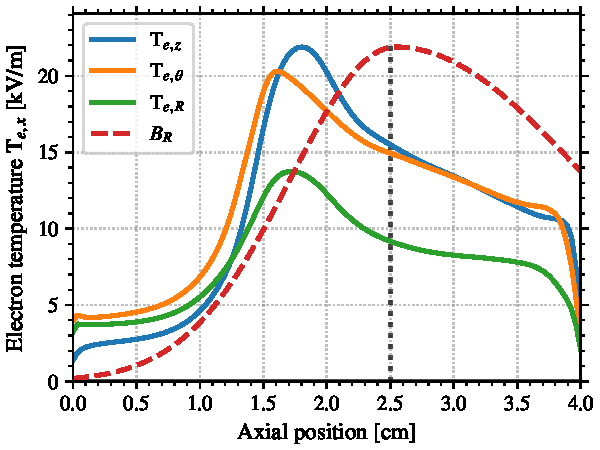
\includegraphics[width=\defaultwidth]{Coches_mean_Tez_profile}
    \caption{ Axial profile of the mean electron temperature in the 3 directions for the case with radial losses.}
    \label{fig-coche-axial-Te}
  \end{figure}
  